\mysubsubsectionformatted{Architettura a strati rilassata}
\myparagraph{
    Come accennato in precedenza, i livelli di un'architettura a layer non comunicano solo con il livello
    sottostante. Si parla quindi di struttura rilassata.

    \begin{center}
        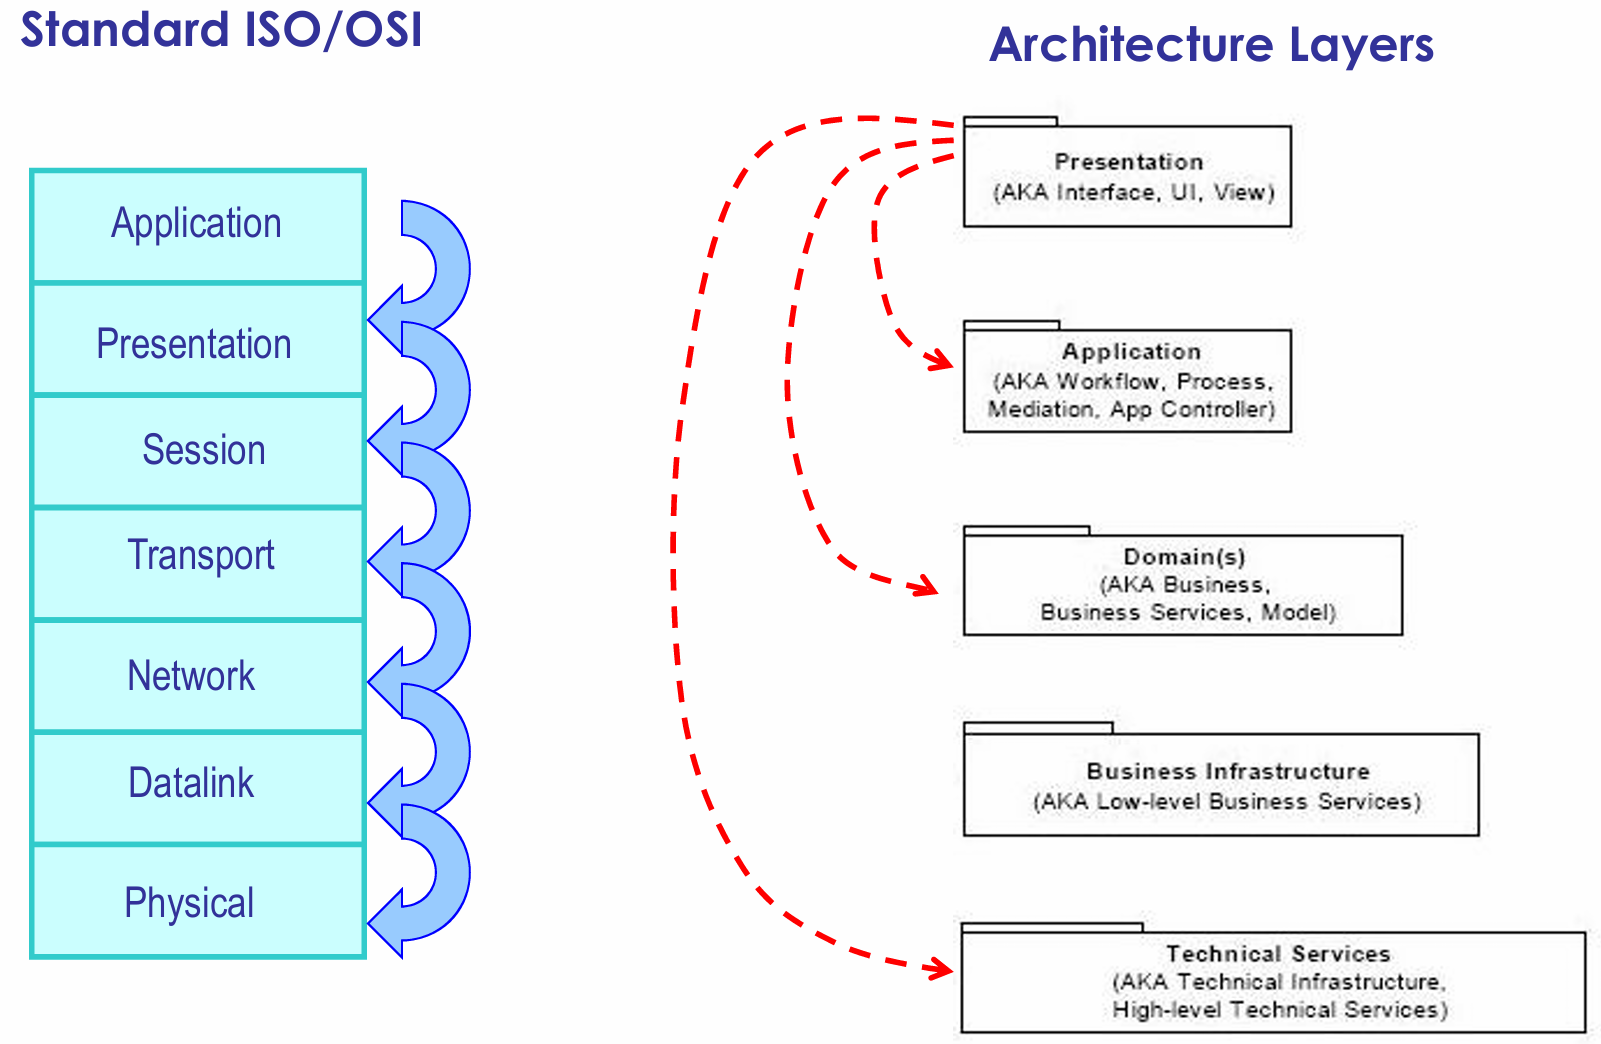
\includegraphics[scale=0.2]{architettura_layer/layer_rilassata.png}
    \end{center}

    \mysubsubsectionformatted{Layer sovrapposti}
    Alcuni oggetti appartengono univocamente a un solo layer.
    \\
    Può capitare che alcuni oggetti, invece, non siano facilmente classificabili, come ad esempio
    i layer Domain e Business Infrastructure oppure Technical Services e Foundation che possono essere
    uniti sotto nome di Infrastructure Layer.

    \newpage
    \mysubsubsectionformatted{Layers e partizioni}
    Generalmente:
    \begin{itemize}
        \item Layers: linee verticali.
        \item Partizioni: divisioni orizzontali.
    \end{itemize}
    Risulta utile distinguerli per diversi motivi:
    \begin{enumerate}
        \item Separation of concerns tra i servizi di alto e basso livello.
        \item Alcuni layers possono essere sostituiti nelle nuove implementazioni.
        \item I layer più bassi implementano funzionalità riutilizzabili.
        \item Viene favorito lo sviluppo in team dal momento che ciascuno sviluppatore è
              specializzato per un layer o servizio definito.
    \end{enumerate}

    \mysubsubsectionformatted{Architettura 3-tier}
    Tipo di architettura che divide il sistema in 3 componenti:
    \vspace{-0.5cm}
    \begin{center}
        \resizebox{\columnwidth}{!}{%
            \begin{tabular}{|l|l|}
                \hline
                \textbf{Interface}         & Interfaccia testuale, GUI e l'interazione diretta con l'utente \\ \hline
                \textbf{Application Logic} & Insieme dei task che governano i processi                      \\ \hline
                \textbf{Storage}           & Meccanismo di memorizzazione persistente (es. Database)        \\ \hline
            \end{tabular}%
        }
    \end{center}

    \begin{center}
        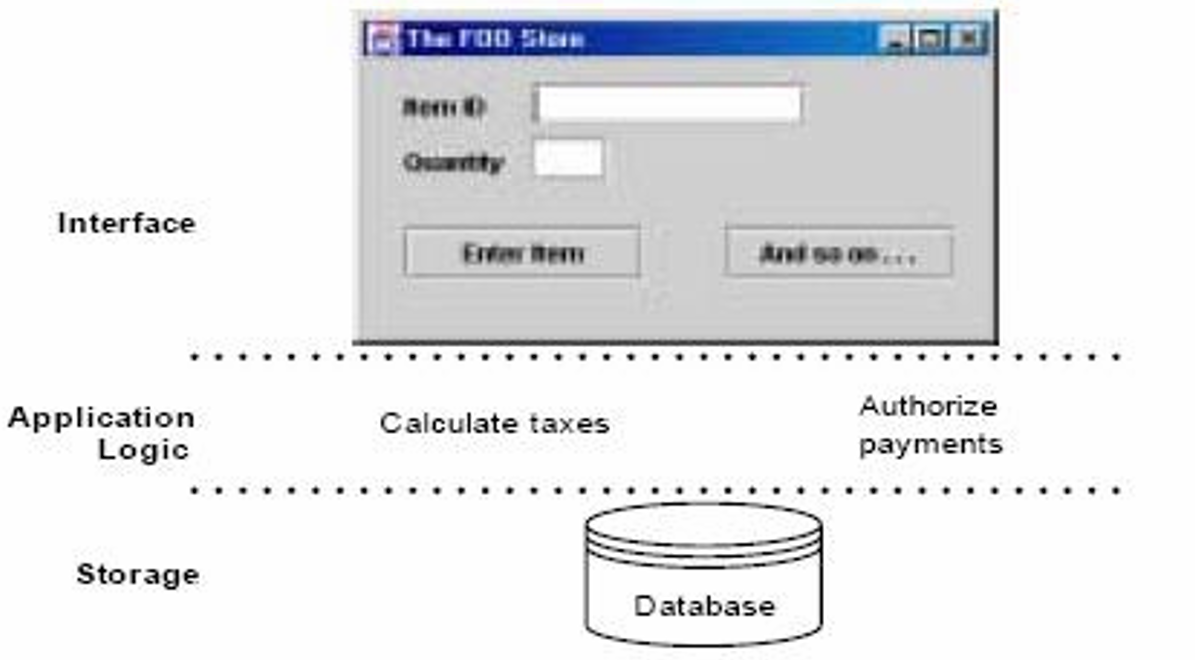
\includegraphics[scale=0.3]{architettura_layer/3tier_archi.png}
    \end{center}
    \newpage
}